\documentclass[11pt]{report}
\usepackage{geometry}
\usepackage{multirow}
\usepackage{array}
\usepackage{xcolor, colortbl}
\usepackage{makecell}
\usepackage{tabularray}
\usepackage[export]{adjustbox}
\geometry{top = 50pt, bottom = 50pt, left = 1in, right = 1in }
\usepackage{graphicx}
\usepackage[T1]{fontenc}
\usepackage{fourier}
\usepackage{setspace}
\usepackage[acronym,shortcuts]{glossaries}
\makenoidxglossaries
\usepackage{url}
\usepackage[hidelinks]{hyperref}

\setlength{\tabcolsep}{18pt}
\renewcommand{\arraystretch}{1.5}

%This is used to control splitting of words using hyphen in LaTeX
\tolerance=9999
\emergencystretch=10pt
\hyphenpenalty=10000
\exhyphenpenalty=100

\loadglsentries{Chapters/abbreviations.tex}

%\rhead{
\includegraphics[width=1cm]{Logo/Thws-logo_English.png}}


%%FOR ADDING HEADER %%%
%\pagestyle{fancy}
%\renewcommand{\chaptermark}[1]{\markboth{#1}{#1}}
%\fancyhead{}
%\fancyhead[L]{\chaptername\ \thechapter\ --\ \leftmark}
%\fancyhead[R]{
\includegraphics[height=0.75cm]{Logo/bosch_logo.png}}
%%\fancypagestyle{plain} %-->To show header on the starting of all Chapters
%\pagestyle{plain}
%\fancyfoot{}
\begin{document}

\pagenumbering{Roman}
\begin{titlepage}
    \par
    
\includegraphics[width=0.3\textwidth, valign=M]{Logo/bosch_logo.png}
    \hfill
    
\includegraphics[width=0.3\textwidth,valign=M]{Logo/Thws-logo_English.png}
    \par
    \vspace{3cm}
    \begin{center}
         \textbf{\Huge Bachelor Thesis}
         \vspace{5pt}
         \\
         for the bachelors degree program in Mechatronics
         \vspace{2.5cm}
         \\
         \textbf{\Huge Development of a Continuous Integration (CI) framework for OptiSlang workflows}
         \vspace{2cm}
         \\
         In co-operation with
         \vspace{5pt}
         \\
         Robert Bosch GmbH
         \vspace{2cm}
         \\
         Author : Sathvick Bindinganavale Srinath\\
         Matriculation Number : 4020025
         \vspace{1cm}\\
         Supervisor : Mr. André Haeitmann Dutra \\
         1\textsuperscript{st} Examiner : \\
         2\textsuperscript{nd} Examiner :
         \vspace{1cm} \\
         Submission Date : 
    \end{center}
\end{titlepage}
%\vspace*{3cm}
\begin{center}
    \textbf{\Huge DECLARATION}
\end{center}
\vspace{2cm}
\begin{onehalfspace}
    I, Sathvick Bindinganavale Srinath, declare that the work in this thesis, \textbf{"Development of a \acrlong{ci} Framework for OptiSlang Workflows"} was carried out in accordance
with the regulations of the Technical University of Applied Sciences Würzburg-Schweinfurt. I have clearly marked and acknowledged all direct quotations and all information obtained from other sources. I have not used any
other sources or resources than those indicated. I have not submitted this thesis to any other examination board.
\end{onehalfspace}

\vspace{1cm}

\vspace*{4em}\noindent
\hfill%
\begin{tabular}[t]{c}
  Ludwigsburg, 05.10.2024\\\rule{10em}{0.4pt}\\ Place, Date
\end{tabular}%
\hfill%
\begin{tabular}[t]{c}
%!Add image of signature here

\includegraphics[width=0.35\textwidth]{Images/signature.pdf}\\\rule{10em}{0.4pt}\\ Signature
\end{tabular}%
\hfill\strut
\tableofcontents
\addcontentsline{toc}{chapter}{List of Figures}
\listoffigures
\addcontentsline{toc}{chapter}{Abbreviations}
\listoftables
\addcontentsline{toc}{chapter}{List of Tables}
{\Large\printnoidxglossary[type=\acronymtype, style=dotlist, title=Abbreviations, nonumberlist]} %nonumberlist prevents adding page number to the glossary.
\cleardoublepage\pagenumbering{arabic}
\begin{spacing}{1.17}

\chapter{Introduction}
\section{Overview}
This thesis explains about the creation and development of a framework for Optislang workflows. The workflow mostly contains modules created using Python and
MATLAB.


\section{Objective}
The objective of this thesis are as follows:
\begin{itemize}
    \item Develop a method to create a standalone version of MATLAB and Python based modules in Optislang for integration testing (only code based, without using 
    \acrshort{gui}).
    \item Implement workflows in batch mode.
    \item Create a framework in Python to create modules and workflows.
    \item Establish a strategy to for automated integration testing in Github for modules based on Python and MATLAB. 
\end{itemize}

\section{Outline}
\begin{itemize}
    \item   In Chapter 2, we are going to discuss about the \acrshort{moo} project, its role in the company and the modules created in Python and Optislang.
    \item   In Chapter 3, we understand the creation of a framework to create standalone modules and workflows in Python.
    \item   In Chapter 4, we will look into the automated integration testing in Github.
    \item   In Chapter 5, we will discuss the results and evaluate the impact of the solution.
    \item   Finally, Chapter 6 provides us the summary of the work, highlighting the achievements and feedback for development in potential areas.
\end{itemize}
\chapter{\acrlong{moo}}

%%%%%%%%%%%%%%%%%   SECTION : INTRODUCTION   %%%%%%%%%%%%%%%%%%%%%%%%%%%%%%
\section{Introduction} \label{what is moo}
In today's increasingly complex world, decision-makers often face the challenge of optimizing several conflicting objectives simultaneously. \acrfull{moo} 
is an optimization that deals with such problems, where multiple objective functions are optimized simultaneously. To understand \acrshort{moo} better, 
let us consider an example.

\paragraph{Example:}
Let us consider an example of a car manufacturer. The car consists of many components like engine, body, wheels, etc which can be
tweaked. In our case, the manufacturer wants to optimize the car for two objectives: lower manufacturing cost of the car and lower carbon emissions. With 
considering the input parameters and the objectives, we get many solutions as shown in Figure \ref{moo}

\begin{figure}[!h]
	\begin{center}
		\input{../Python/plots/moo_plot.tex}
	\end{center}
    \caption{Example of \acrshort{moo}}
    \label{moo}
\end{figure}
In an \acrshort{moo} problem, there typically is no single best solution. Rather, the \textit{goal} is to identify a set of solutions that are optimal in terms 
of all objectives. In Figure \ref{moo}, the best solutions for the given objectives is indicated in orange known as pareto optimal solutions. A solution is said 
to be pareto optimal if no other solution can improve on any of the objectives without worsening at least one of the other objectives.
%The solutions which are not Pareto optimal are not considered as they are dominated by the Pareto optimal solutions. 

\section{Difference between \acrshort{moo} and \acrshort{soo}}
Optimization problems, whether single-objective or multi-objective, have the same goal: to find the best solution(s) to a given problem. However, the approach
to solving these problems is different. 

In \acrfull{soo}, the goal is to optimize a single objective function, which can either be maximized or minimized. The  problem is simpler to define and solve
because it involves only one objective. To calculate \acrshort{soo}, we can use methods like gradient descent, linear programming, etc.

\begin{figure}[!h]
    \centering
    \input{../Python/plots/soo_plot.tex}
    \caption{Example of \acrshort{soo}}
    \label{soo}
\end{figure}

In Figure \ref{soo}, we have considered the same example given in section \ref{what is moo}. But, here, we are considering only one objective, which is to
minimize the manufacturing cost. The best solution is indicated in orange.
\vspace{15pt}

In \acrshort{moo}, the optimization involves two or more objective functions simultaneously. The problem is more complex because the objectives are often
conflicting. Unlike \acrshort{soo}, where we have a single best solution, in \acrshort{moo}, we have pareto optimal solutions.
To calculate \acrshort{moo}, we can use methods like pareto optimization, scalarization method, weighted sum method, $\epsilon$-constraint method, etc.


While \acrshort{soo} focuses on finding the best solution according to a single criterion, \acrshort{moo} addresses the more complex task of balancing multiple, 
often conflicting objectives. The choice between \acrshort{soo} and \acrshort{moo} depends on the nature of the problem at hand and the goals of the decision-maker. 
Understanding the differences between these approaches is crucial for selecting the appropriate optimization technique and achieving the desired outcomes.

%%%%%%%%%%%%%%%   SECTION : OPTISLANG  %%%%%%%%%%%%%%%%%%%%%%%%%%%%%%%%
\section{Optislang}
\paragraph{}

To calculate \acrshort{moo}, we need a software platform that can handle the complexity of the problem. Ansys Optislang \cite{optislang} is such a software 
platform, which is used for design exploration, \acrfull{cae} based sensitivity analysis and optimization in conjunction with any product development tool. 
It is a Process Integration and Design Optimization tool or in short, a \acrshort{pido} tool. Process Integration refers to automate and orchestrate manual 
simulation processes and to realize complex workflows. Design Optimization aims for better understanding of your design, optimizing the product, identify an 
improved design which has the desired qualities and resulting in a best design by reliability analysis and statistical analysis.  


Optislang uses several solvers to look into aspects like mechanical, technical, mathematical and any other problems. This is easier in Optislang as it provides
integration to create toolchains of many external programs like ANSYS, MATLAB, Excel, Python, CATIA and many more.


Our department utilizes Optislang for solving \acrshort{moo} problems, as it includes algorithms specifically designed for \acrshort{moo}.
%# Try to explain about the parametric system, sensitivity analysis, MOP, ...
%%%%%%%%%%%%%%%%%   SECTION : MODULES AND WORKFLOWS   %%%%%%%%%%%%%%%%%%%%%%%%%%%%%%
\section{Modules and Workflows}
\subsection{Modules}
Modules are created by the system developers. Modules include a simulation model as a calculation with defined interfaces for coupling with other modules. 
These modules are either defined in MATLAB or Python. Each module is designed to tackle/improve a specific issue. To document and collaborate with other
system developers, each module is versioned and stored in a specific manner in a repository in GitHub Enterprise.

\begin{figure}[!h]
    \centering
    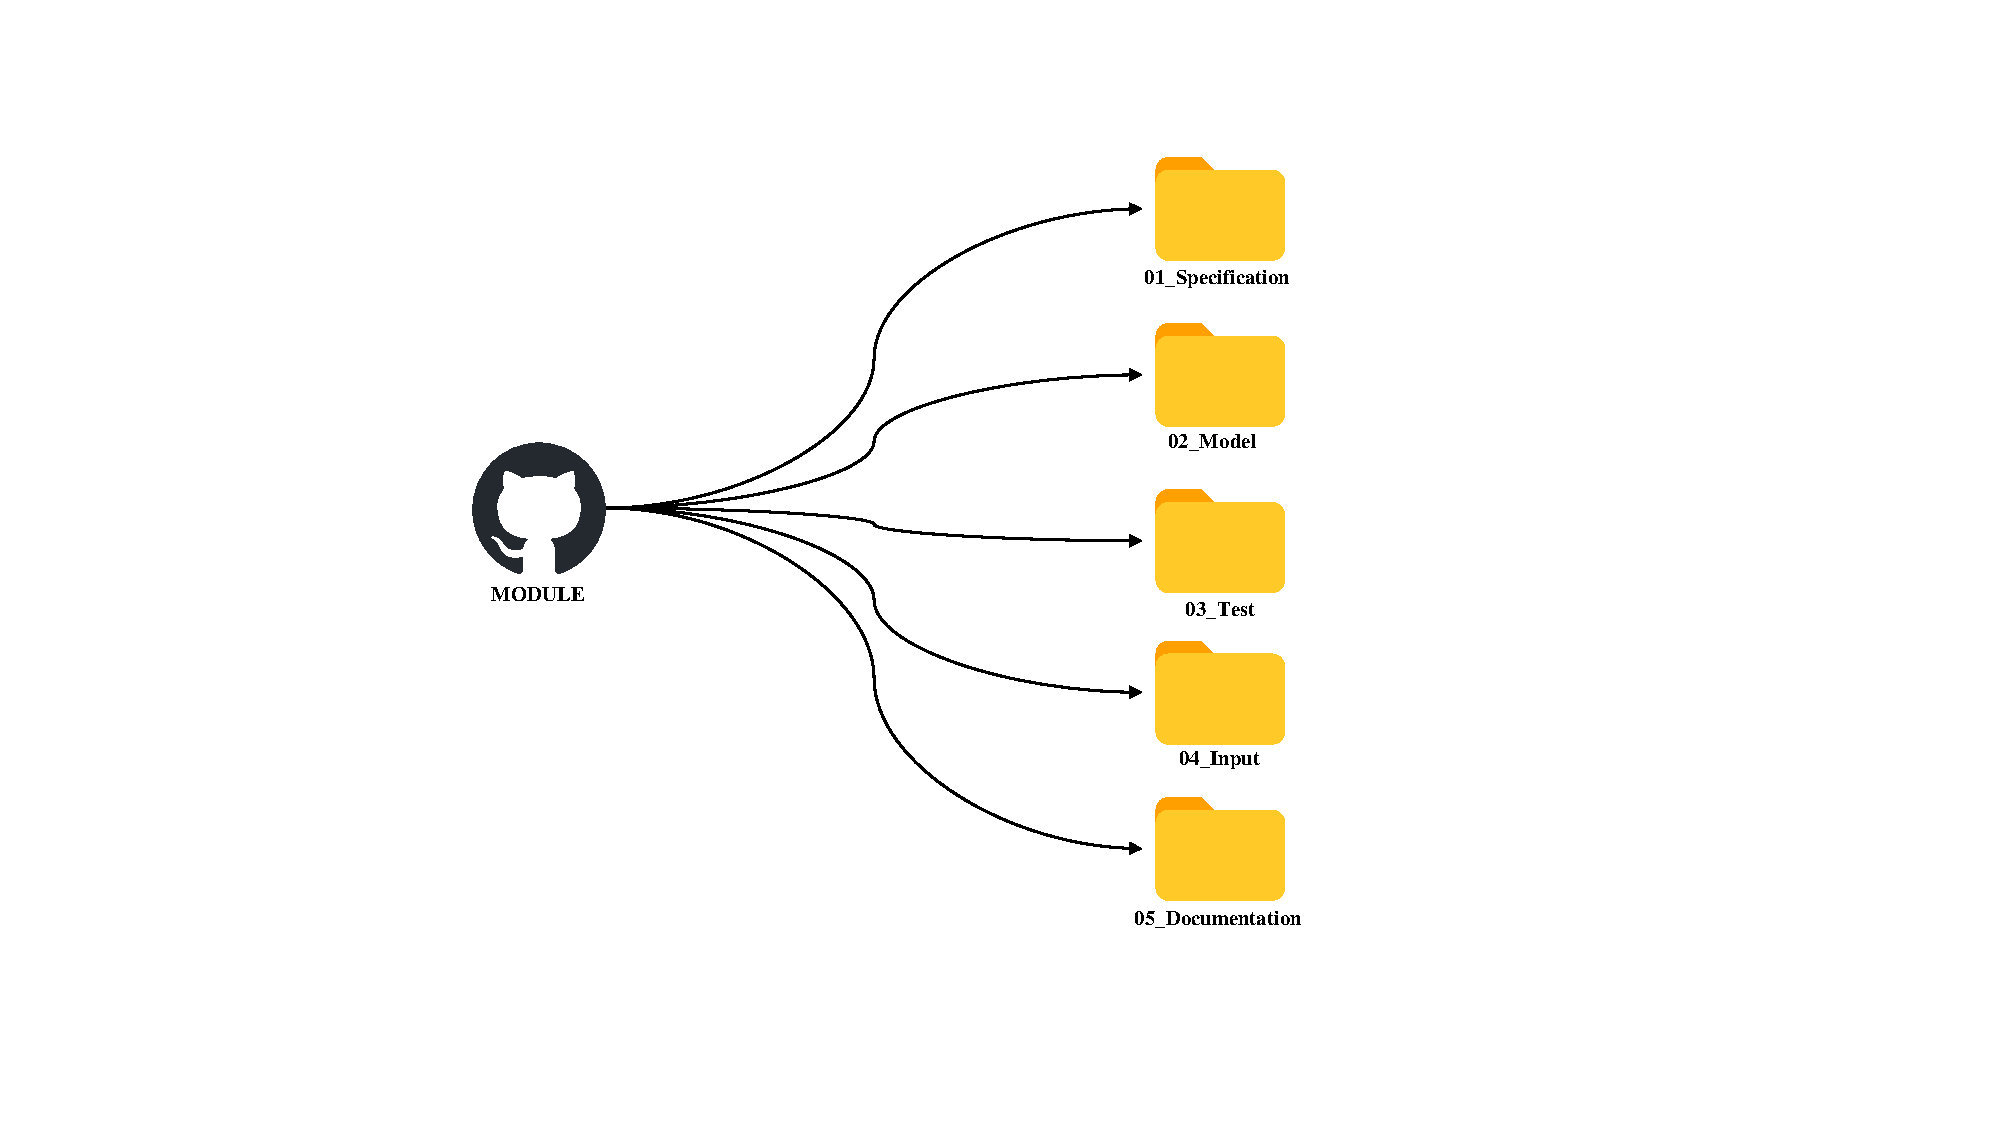
\includegraphics[width=1.2\textwidth]{Images/github_folder_structure.pdf}
    \caption{Example of a module's GitHub repository structure}
    \label{github_arrhenius}
\end{figure}

Figure \ref{github_arrhenius} shows us an example of how each module is maintained in our GitHub organization.
\begin{itemize}
    \item \verb|01_Specification| has all the requirements for the module to run.
    \item \verb|02_Model| contains all parts to run the model. This can also be used as a playground for the development of a model.
    \item \verb|03_Test| contains all the unit tests for the module. This is to ensure that the module is working as expected.
    \item \verb|04_Input| carries all the initial parameters or functions to be defined at the start of a module.
    \item \verb|05_Documentation|contains documents explaining functioning and usage of the module.
\end{itemize}
%\begin{table}[!h]
%    \begin{tabular}{|>{\centering\arraybackslash}p{2cm}|>{\centering\arraybackslash}p{12cm}|}
%        \hline
%        Name of the module & \multirow{2}{*}{\centering Use Case}\\
%        \hline
%        Pv Calculator & Simulation of FET losses as input for the FET's temperature estimation as base for a first reliability prognosis\\
%    \end{tabular}
%\end{table}
\subsection{Workflows}
Our department develop automatized workflows for power electronics products considering functional loads to reliability indications. Workflows are a sequence
of modules designed for a fast calculation performance characteristic like temperature or reliability indication. To develop a workflow, Optislang is used.


Every architectural workflow has a GitHub repository that is maintained in a similar way to how modules are being maintained.

\begin{figure}[!h]
    \centering
    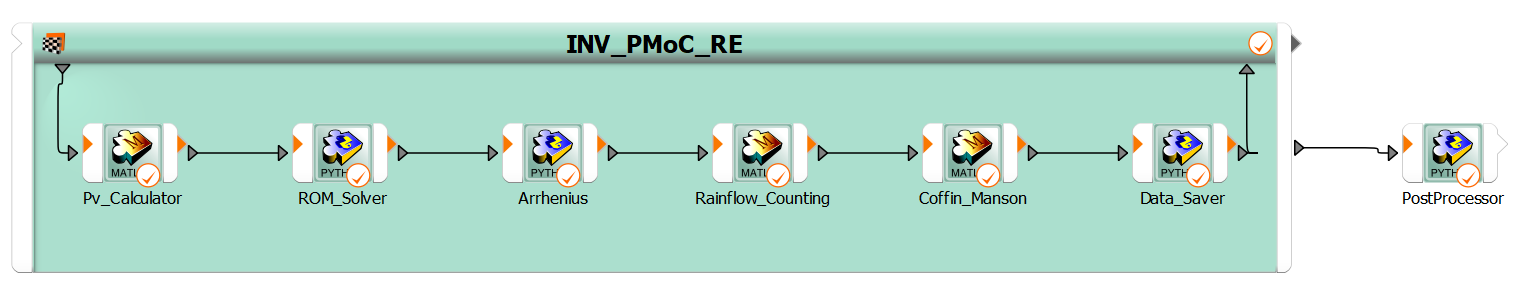
\includegraphics[width=\textwidth]{Images/workflow_example.png}
    \caption{Example of a workflow in Optislang}
    \label{workflow_example}
\end{figure}

%%%%%%%%%%%%%%%%%   SECTION : CURRENT PROBLEM   %%%%%%%%%%%%%%%%%%%%%%%%%%%%%%
\section{Current Problem} \label{current problem}
lorem ipsum dolor sit amet, consectetur adipiscing elit. Donec auctor, nunc nec lorem ipsum dolor sit amet, consectetur adipiscing elit. Donec auctor, nunc
nec lorem ipsum dolor sit amet, consectetur adipiscing elit. Donec auctor, nunc nec lorem ipsum dolor sit amet, consectetur adipiscing elit. Donec auctor, nunc
nec lorem ipsum dolor sit amet, consectetur adipiscing elit. Donec auctor, nunc nec lorem ipsum dolor sit amet, consectetur adipiscing elit. Donec auctor, nunc
nec lorem ipsum dolor sit amet, consectetur adipiscing elit. Donec auctor, nunc nec lorem ipsum dolor sit amet, consectetur adipiscing elit. Donec auctor, nunc
nec lorem ipsum dolor sit amet, consectetur adipiscing elit. Donec auctor, nunc nec lorem ipsum dolor sit amet, consectetur adipiscing elit. Donec auctor, nunc
lorem ipsum dolor sit amet, consectetur adipiscing elit. Donec auctor, nunc nec lorem ipsum dolor sit amet, consectetur adipiscing elit. Donec auctor, nunc
nec lorem ipsum dolor sit amet, consectetur adipiscing elit. Donec auctor, nunc nec lorem ipsum dolor sit amet, consectetur adipiscing elit. Donec auctor, nunc

 %#! Explain why it is time consuming to test the module, labour intensive, increase of errors with complexity of the module/workflow
 %#! Explain the lack of standardization of module, difficulty in maintaining the modules effectively
\chapter{Application of my Thesis}

To overcome the problems discussed in section \ref{current problem}, this thesis proposes a solution to automate the process of testing standalone modules
in Optislang. Since, the process is automated, the testing of modules needs to be done without the help of the \acrshort{gui}. To achieve this, a Python
\cite{python} framework is created to test the modules in an according manner. To use the framework in an automated manner, a \acrshort{ci} pipeline is created using GitHub Actions. The pipeline 
is triggered whenever a new commit is pushed to the repository. The pipeline runs the tests on the modules in a virtual machine and checks if the results are as expected. If the tests 
fail, the pipeline notifies the developer about the failure. The developer can then look into the issue and resolve it.

\section{DevOps}
Devops is the combination of a set of practices, tools which helps to automate and integrate the processes between software and organizations.

DevOps practices play a crucial role in the development of the automation process described in this thesis. By integrating \acrfull{ci} and \acrfull{cd} pipelines, we ensure that the testing of 
modules is efficient and reliable. This helps us to improve productivity and reduce human error. The DevOps approach allows for seamless collaboration between development and operations teams, 
ensuring that the testing framework and the modules it tests are consistently maintained and updated. This integration of DevOps practices not only enhances the quality of te software but also 
accelerates the development lifecycle, enabling faster delivery of new updates and features.
\begin{figure}[!h]
    \centering
    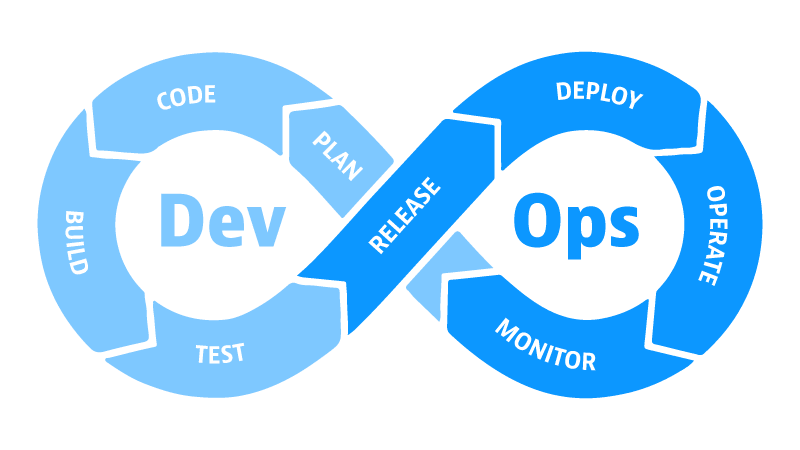
\includegraphics[width=0.7\textwidth]{Images/devops_loop.png}
    \caption{DevOps lifecycle}
    \label{devops_lifecycle}
\end{figure}

In summary, the application of DevOps in this thesis demonstrates how modern software engineering practices can be applied to automate and streamline the testing process, leading to more robust,
efficient and reliable software solutions.

\section{\acrfull{ci}}

\section{Code quality}
\chapter{Creation of a \acrshort{ci} Framework}
%Create a flowchart explaining the steps in the framework
%Explain each section in detail
%Explain creation of retrieving the input files using FAST API and OpenShift
%Explain storing of the framework in GitHub
\bibliographystyle{plain}
\bibliography{Chapters/references.bib}
\end{spacing}

\end{document}